\chapter{Prerequisites}

- To localize a whistle sound source, it must be detected firstly (was done by previous work
and is implemented)
- calculate the direction of the whistle sound on one Nao\\
- This can be done by determining the \ac{TDOA} of microphone pairs\\
- With the delay, the angle of the sound source relative to angle pair
can be is known.\\
- By combining these, a direction ray is defined on each Nao\\
- The results are filtered by updating it with the singe rays, assuming
gaussian distribution. (known error, Trigonometry)

- why other theories do not fit into this problem
(finger printing, beam forming)

- CC in time domain, because low frequency resolution (44100Hz/512Samples=resolution)
and also \ac{CC} corrupted and we want to detect which signal was first
- reverberation is a problem and assumed as not multi-path system

\missing[inline]{more content}

\section{Whistle Signal}
\label{sec:02_whistleSignal}

In this work the localization of a whistle sound source is to be to the fore.
The detection of such a signal is implemented as stated in \cite{Hasselbring}.\\
- short explanation of how the whistle is detected\\
- whistle sound is around 2000Hz and 4000Hz

Further on, the mathematical model of a received whistle signal at one microphone sensor
is defined as
\be
x(t) = s(t) + n(t)
\label{eq:02_whistleSignal}
\ee
where $s(t)$ represents the signal and $n(t)$ noise.
Both are real, jointly stationary random processes.
\section{Time Difference Of Arrival}
\label{sec:02_tdoa}

The direction of a signal source $\gamma'$ can be detected by the time delay of
the received signal.
Calculations for the direction of the sound source can be done with a
geometrical approach like in \cite{Valin_Michaud}.
\Cref{fig:02_tdoa} illustrates the delay introduced by the direction angle
of the sound source relative to a vector between channels 0 and 1.
If the delay is zero, the signal is perpendicular to this channels vector.
It's value can be $s_{max}$ maximally which delivers the result that the source
direction must be aligned to the channels vector direction.
It is assumed that the distance from the sensors to the sound source is
significantly large so that the signal waves proceed parallel which is a necessary
criterion for the approach to be valid.
\begin{figure}[ht]
	\centering
		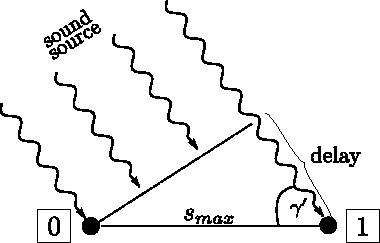
\includegraphics[width=0.4\columnwidth]{figures/tdoa_waves}
	\caption{Illustration of TDOA principle.}
    \label{fig:02_tdoa}
\end{figure}
% -------------------------------------------------------------

Specifying the speed of sound $c_s$ being 343\si{m/s} in air, the angle
$\gamma'$ can be defined as
\bsub \bal
    \gamma' &= cos^{-1}(\frac{|delay|}{s_{max}})
    \label{eq:02_tdoaAngle}\\
    \intertext{with}
    s_{max} &= \frac{f_s * d_{max}}{c_s}
\eal \esub
where $f_s$is the sampling rate.
% -------------------------------------------------------------

With the definition of a whistle signal as stated in \cref{eq:02_whistleSignal},
the microphone sensors $mic_1$ and $mic_2$ will output
\bsub \bal
    x_1(t) &= s(t) + n_1(t)\\
    x_2(t) &= \alpha s(t - D) + n_2(t).
\eal \esub
\label{eq:02_signalTimeDomain}
Here, $D$ is the delay of $x_2$ relative to $x_1$ for which is looked for.
\section{Cross Correlation}
\label{sec:02_cc}

The \ac{CC} provides information about the similarity of two signals.
Thus, the delay of one signal can be detected where the \ac{CC} function $R_{x_0x_1}(t)$ is largest.
% -------------------------------------------------------------
In time domain, the \ac{CC} of two signals $x_0$ and $x_1$ is denoted as
\bal
    R_{x_0x_1}(t) = \int^{+\infty}_{-\infty}x_0(\tau-t)x_1(\tau)d\tau.
\eal
Considering the frequency domain, the function can be transformed into
\bal
    \mathcal{F}[R_{x_0x_1}(t)] = G_{x_0x_1}(f) = X_0^*(f)X_1(f)
    \label{eq:02_ccBaseFunction}
\eal
with $\mathcal{F}[x_i(t)] = X_i(f)$ and $X_i^*(f)$ indicating the conjugate complex form.
% -------------------------------------------------------------
However, the finite observation time of the received signal corrupts the fourier
transform \cite{K_C_GCC}
and noise of sensors may introduce false peaks in the \ac{CC} \cite{H_B_GCC}.
% -------------------------------------------------------------
In frequency domain, the signals $x_0(t)$ and $x_1(t)$ from \cref{eq:02_signalTimeDomain}
can be expressed as
\bsub
\label{eq:02_signalFreqDomain}
\bal
    X_0(f) &= S(f) + N_0(f)\\
    X_1(f) &= \alpha S(f) e^{-j2\pi fD}+ N_1(f).
\eal \esub
% -------------------------------------------------------------
Thus, the \ac{CC} is
\bsub
\label{eq:02_Gx0x1}
\bal
    G_{x_0x_1}(f) &= \alpha |S(f)|^2 e^{-j2\pi fD} + N_0^*(f)N_1(f) + S^*(f) N_1(f) + \alpha S(f) e^{-j2\pi fD}N_0^*(f)\\
\intertext{which will be shortened as}
    G_{x_0x_1}(f) &= \alpha \phi_s(f) e^{-j2\pi fD} + \phi_n(f) + \phi_c(f) \label{eq_02_Gx0x1_simple} \\
\intertext{where}
\phi_s(f) &= |S(f)|^2 \label{eq:02_phi_s} \\
\phi_n(f) &= N_0^*(f)N_1(f) \label{eq:02_phi_n1n2} \\
\phi_c(f) &= S^*(f) N_1(f)+\alpha S(f)e^{-j2\pi fD}N_0^*(f) \label{eq:02_phi_c}.
\eal \esub
%\cite{H_B_GCC}
% -------------------------------------------------------------
Considering the ideal case where $s(t)$, $n_0(t)$ and $n_1(t)$ are uncorrelated, the terms
$\phi_c$ and $\phi_n$ disappear and the \ac{CC} results in
\bal
    R_{x_0x_1}(t) = \mathcal{F}^{-1}[\alpha \phi_s(f) e^{-j2\pi fD}] = \alpha \mathcal{F}^{-1}[\phi_s(f)] * \delta(t-D).
    \label{eq:02_R12_noNoise}
\eal
In general, $\phi_c$ and $\phi_n$ can neither be neglected nor assumed as uncorrelated to the signal \cite{H_B_prob},
so that they introduce inaccuracies and errors.

% -------------------------------------------------------------
% \unsure[]{do I fully understand this? Is this correct?}
% This means there exists a peak at delay $D$ which is altered by the \ac{iFT}
% of the signal spectrum.
As introduced, the \ac{CC} gives insight about the similarity of two signals and at peak, they
are most alike.
Received signals from microphone sensors are digital signals sampled with a certain
frequency.
The derivations are just as applicable, but transformations into frequency
domain are done by \ac{DFT}.
In the case of real data samples with length $n$ and similar \ac{DFT} size, the shift between
the zero index and the peak is the resulting delay $D$.
Zero index is defined as the index of the peak if no shift exists.
% -------------------------------------------------------------

\Cref{fig:03_ccTheory} is the outcome of two similar, but shifted sine signals with
3\si{\kilo\hertz} and normally distributed noise.
As the second signal is delayed by 10 samples, the peak can be detected where $shift = 10$.
The example signals are attached in \cref{fig:ap1_signals}.
One disadvantage of this technique is that for periodic signals the \ac{CC} also is periodic
and the peak is not always easily detectable. Noise and inaccuracies of the \ac{FFT} then
may influence the result what can make the peak unobvious \cite{L_L_GCC}.
\begin{figure}[ht]
	\centering
		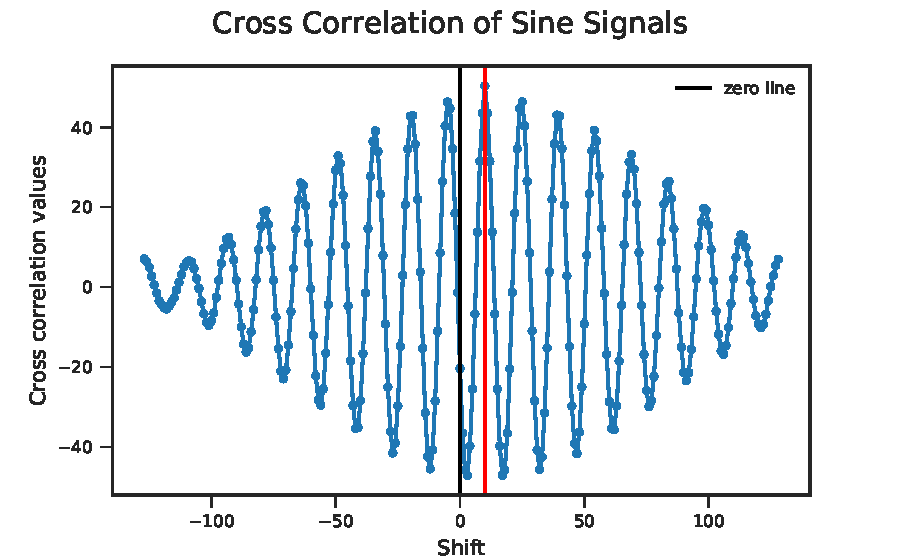
\includegraphics[width=1\columnwidth]{figures/CC_theory}
	\caption{Cross correlation of two generated sine signals with 3\si{\kilo\hertz}.}
    \label{fig:03_ccTheory}
\end{figure}

\section{Generalized Cross Correlation}
The generalized cross correlation is super duper nice.

\section{Signal Start Detection}
\label{sec:02_signalStartDetection}

One focus of the whistle signal localization is the correct choice of the
signal frame, with which the \ac{TDOA} measurement is done.
In order to perform the \ac{FFT} most efficiently, the size of one frame
should be a power of 2.
Assuming that the clearest signal without reverberation and with minimal
multipath propagated subsignals is at the start of a sound signal,
the frame to investigate is chosen to be at the beginning of a whistle sound.
Several methods exist and can be combined at will.
In the next subsections, signal start detection using entropy, energy and
zero crossing rate are subject of discussion.

\subsection{Entropy}
%\section{Signal Phase Difference}
\label{sec:02_phase}

With a different approach to the correlation methods, the \ac{TDOA} can be
detected by observing the phase of one reference frequency $f_c$.
Imaging a single-sinusoidal signal moving from left to right as
pictured in \cref{fig:02_phaseTheory}, two distant sensors
(\textit{channel 2} and \textit{channel 3}) will
receive different parts of the signal at the same time.
Transforming the frames into frequency domain by \ac{FFT}, the pase of the
maximal frequency differ by the delay.
% -------------------------------------------------------------

\begin{figure}[ht]
	\centering
		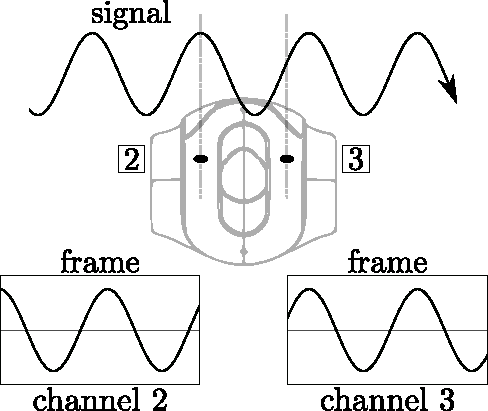
\includegraphics[width=0.35\columnwidth]{figures/phase_theory}
	\caption{Explanatory illustration of the phase difference method.}
    \label{fig:02_phaseTheory}
\end{figure}
% -------------------------------------------------------------

The phase of a signal's reference frequency is easily computable in frequency domain
with
\bal
    \phi(f_c) &= tan^{-1}\left(\frac{imag(X(f_c))}{real(X(f_c))}\right).
\eal
% -------------------------------------------------------------
With the difference of the phases of two channel, the delay in meters is defined as
\bal
    D &= \frac{\Delta \phi \cdot c_s}{2 \pi \cdot f_c}.
\eal
From that, the direction angle calculation of \cref{eq:02_tdoaAngle} can
be followed.
It should be noted that certain requirements needs to be fulfilled to receive a
unambiguous result due to signal periodicity.
\Cref{subsubsec:03_phase} covers the conditions that apply for this thesis's
hardware.
% -------------------------------------------------------------
%\input{content/02_Trigonometry}

%\input{content/02_filter}
